\documentclass[10pt,a4paper]{article}
\usepackage[utf8]{inputenc}
\usepackage{amsmath}
\usepackage{amsfonts}
\usepackage{amssymb}
\usepackage{color}
\usepackage{graphicx}
\usepackage[dvipsnames]{xcolor}
\usepackage{fancyhdr}
\usepackage{parskip}
\usepackage{anysize}
\author{Fabio Víctor Alonso Bañobre}
\title{Informe Moogle}

 

\begin{document}  
\marginsize{2cm}{2cm}{2cm}{2cm}

\begin{figure}[t]
	\centering
	\includegraphics{moogleTítulo.png}
\end{figure}

\textcolor{White}{\colorbox{NavyBlue}{OBJETIVO DE ESTUDIO}}\\

MOOGLE es una aplicación web que permite realizar una búsqueda en archivos TXT de una o 
varias palabras. Como resultado de la búsqueda, se listan los nombres de los ficheros que 
contengan al menos una palabra de la frase.
Los ficheros se listan en orden descendente, mostrando al inicio los que contengan mayor 
ocurrencia de la(s) palabra(s) a buscar.\\

\textcolor{White}{\colorbox{NavyBlue}{DESCRIPCIÓN DE LAS CLASES}}\\


\underline{Clase: \textbf{Query}}\\

En esta clase se definen las propiedades y métodos para trabajar con la query. 
Dictionary<int, string> dicWordsOfQuery: diccionario que almacena cada palabra de la query.
countwordsInQuery: propiedad que almacena la cantidad de palabras de la query\\

CleanQuery: método que
 Elimina los espacios en blanco que existan al inicio y fin de la query\\
\begin{itemize}

\item Convierte a minúscula los caracteres de la(s) palabra(s) de la query.

\item Elimina los caracteres especiales que pueda tener la query.

\item Maneja los acentos que pudiera tener alguna palabra de la query.

\item Elimina las conjunciones, preposiciones y artículos de la query.\\
\end{itemize}

FillDictionaryQuery: método que actualiza el diccionario dicWordsOfQuery con las palabras de
la query\\

\underline{Clase: \textbf{FilesTXT}}\\

En esta clase se definen las propiedades y métodos para trabajar con los ficheros TXT.\\
 
Dictionary<int, string> dicFilesTxt: diccionario que almacena el nombre de cada archivo TXT\\

Dictionary<int, string> dicFilesSnippet: diccionario que almacena una cadena de caracteres del 
TXT donde aparezca la(s) palabra(s) de la query\\

countFilesTxt: propiedad que almacena la cantidad de ficheros TXT que se encuentran en la 
carpeta Content\\

FillDictionaryTXT: método que actualiza el diccionario dicFilesTxt con los nombres de los 
archivos TXT y el diccionario dicFilesSnippet\\

\underline{Clase: \textbf{TFIDF}}\\

Esta clase contiene las siguientes propiedades y métodos.\\

double[,] mtzGeneral: matriz cuya cantidad de filas se corresponde con la cantidad de archivos 
TXT y la cantidad de columnas se corresponde con la cantidad de palabra(s) de la query. Cada 
elemento de la matriz contiene la cantidad de veces que se encuentra cada palabra de la query
en cada TXT.\\

double[,] mtzGeneralTFIDF: matriz cuya cantidad de filas se corresponde con la cantidad de 
archivos TXT y la cantidad de columnas se corresponde con la cantidad de palabra(s) de la query. 
Cada elemento de la matriz contiene el valor calculado de TF * IDF\\

double[] arrayQueryTF: la cantidad de elementos de este arreglo se corresponde con la cantidad 
de palabra(s) de la query. El valor que almacena cada elemento del arreglo es el valor calculado 
de TF para cada palabra de la query.\\

double[] arrayQueryIDF: la cantidad de elementos de este arreglo se corresponde con la 
cantidad de palabra(s) de la query. El valor que almacena cada elemento del arreglo es el valor 
calculado de IDF para cada palabra de la query.\\

double[] arraySimCoseno: la cantidad de elementos de este arreglo se corresponde con la 
cantidad de archivos TXT y cada valor del arreglo contiene el valor calculado de la similitud 
coseno.\\

FillMatrizGeneral: método que actualiza la matriz mtzGeneral\\

FillMatrizTFIDF: método que actualiza la matriz mtzGeneralTFIDF\\

UpdateArrayQueryTF: método que actualiza el arreglo arrayQueryTF\\

UpdateArrayQueryIDF: método que actualiza el arreglo arrayQueryIDF\\

UpdateSimilitudCoseno método que actualiza el arreglo arraySimCoseno\\

**La aplicación tenía definida previamente las clases: SearchItem y SearchResult **\\

\textcolor{White}{\colorbox{NavyBlue}{DESCRIPCIÓN DEL FUNCIONAMIENTO DE LA APLICACIÓN}}\\

La carpeta donde se encuentra la solución de la aplicación tiene una subcarpeta denominada: 
Content , y es en ella donde deben estar ubicados los archivos TXT.\\

El usuario, al teclear la(s) palabra(s) a buscar, que le hemos estado llamando: query, los procesos 
que se ejecutan son:\\
\begin{enumerate}
\item Limpiar la query: los caracteres de la query se convierten a minúsculas; se eliminan los 
caracteres especiales y estructuras del idioma como: las conjunciones, preposiciones, 
artículos; se eliminan los espacios al inicio y fin de la query, se manejan los acentos.\\

\item Recorrer la lista de palabras de la query y almacenar cada palabra en el diccionario 
dicWordsOfQuery\\

\item Recorrer la lista de archivos TXT que se encuentran en la carpeta Content y almacenar 
cada nombre del archivo TXT en el diccionario dicFilesTxt\\

\item Determinar la ocurrencia (cantidad de veces) que se encuentra cada palabra de la query
en cada archivo TXT. Estas cantidades se almacenan en la matriz mtzGeneral.\\

\item Calcular para cada palabra de la query, el valor de TF y almacenarlo en el arreglo 
arrayQueryTF\\

\item Calcular para cada palabra de la query, el valor de IDF y almacenarlo en el arreglo 
arrayQueryIDF\\

\item Tomando en cuenta los valores calculados anteriormente de TF y de IDF, actualizar la 
matriz mtzGeneralTFIDF\\

\item Calcular la similitud coseno y salvar los datos calculados en el arreglo arraySimCoseno\\

\item Recorrer el arreglo arraySimCoseno para actualizar la estructura SearchItem\\

\item El contenido de SearchItem es lo que se muestra en la pantalla como resultado de la 
búsqueda realizada.\\
\end{enumerate}

\newpage
\textcolor{White}{\colorbox{NavyBlue}{EJEMPLO DE EJECUCIÓN DE LA APLICACIÓN}}

\begin{figure}[h]
	\centering
	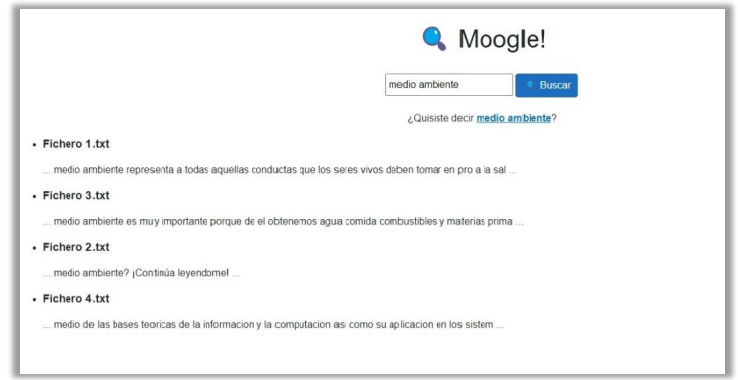
\includegraphics{mooglePaint.png}
	\caption{Funcionamiento Moogle}
\end{figure}

\end{document}